% Template for ICME-2010 paper; to be used with:
%          spconf.sty  - ICASSP/ICIP LaTeX style file, and
%          IEEEbib.bst - IEEE bibliography style file.
% --------------------------------------------------------------------------
\documentclass{article}
\usepackage{spconf_ICME,amsmath,epsfig,fancyhdr}
\setlength{\paperwidth}{215.9mm} \setlength{\hoffset}{-9.7mm}
\setlength{\oddsidemargin}{0mm} \setlength{\textwidth}{184.3mm}
\setlength{\columnsep}{6.3mm} \setlength{\marginparsep}{0mm}
\setlength{\marginparwidth}{0mm} \setlength{\paperheight}{279.4mm}
\setlength{\voffset}{-7.4mm} \setlength{\topmargin}{0mm}
\setlength{\headheight}{0mm} \setlength{\headsep}{0mm}
\setlength{\topskip}{0mm} \setlength{\textheight}{235.2mm}
\setlength{\footskip}{12.4mm} \setlength{\parindent}{1pc}


\ICMEfinalcopy % *** Uncomment this line for the final submission
\def\ICMEPaperID{}
\def\httilde{\mbox{\tt\raisebox{-.5ex}{\symbol{126}}}}

% Pages are numbered in submission mode, and unnumbered in camera-ready
\ifICMEfinal\pagestyle{empty}\fi


\begin{document}\sloppy

% Title.
% ------
\title{AUTOMATICALLY DISTINGUISHING BETWEEN SUNSET AND NON-SUNSET SCENES USING MACHINE LEARNING}
%
% Single address.
% ---------------
\name{Nicholas Kamper and Eric Henderson}
\address{Rose-Hulman Institute of Technology \\
Email: kampernj@rose-hulman.edu and henderea@rose-hulman.edu}


\maketitle
% insert page header and footer here for IEEE PDF Compliant
\thispagestyle{fancy} \fancyhead{} \lhead{}
\renewcommand{\headrulewidth}{0pt}
\renewcommand{\footrulewidth}{0pt}




%
\begin{abstract}
Scene detection is a complicated problem with many commercial applications in 
consumer products. For this paper, we implemented detection of sunset versus 
non-sunset scenes using  support vector machine
\end{abstract}

%
\begin{keywords}
sunset detector,scene classification,support vector machine,image classification
\end{keywords}

%
\section{Introduction}
\label{sec:intro}
For the sunset detector project, we set out to devise an accurate way to classify
whether a given image is a sunset or not using supervised machine learning techniques.

Scene classification has several practical applications. One such use is in consumer
imaging devices to determine the best post-processing steps to deliver a high quality
image. Another would be automated image sorting based on the scene type (e.g., being 
able to classify portraits, nature shots, and so on, to categorize them in an album). 

Scene classification is difficult, even in the binary case that we consider in this
paper. Certain scenes would be very difficult to classify, as they would share the
same characteristics, such as hue and brightness features, as other scenes.

\section{Problem Description}
\label{sec:probdesc}
In this particular scenario, we wanted to develop a classifier that would give a binary
classification as to whether a scene contained a sunset or not, only using a set of 
approximately 500 training images.  

\section{Implementation}
To solve this problem, we started out by implementing a baseline detector. First, we converted the source image to the LST (luminance and chroma) bands. Once in LST, to obtain the feature vector, we split the image into a 7x7 equidistant grid and took the mean and standard deviation of each of the LST bands for each of the 49 regions. This resulted in a 294 dimension feature vector for each image. 

The feature vector was then normalized using the zero-mean and one-standard deviation method. With the 294 dimension normalized training feature vector, we trained an SVM using several different kernels, both polynomial and radial basisfunction kernels, varying the kernel parameter to obtain the best accuracy. 

After training the SVM, we then ran the SVM on a set of test data, obtaining a set of labels. We then normalized those labels using the same zero-mean and one-standard deviation method and used a threshold of 0 to assign integer labels to each image. We compared the results of various kernels and parameters to obtain the best results. 

In an attempt to improve our accuracy, in addition to normalizing the Y1 label values from the SVM, we also tried varying the grid size. However, this technique did not result in any improvements to the accuracy over the baseline 7x7 grid. 

\begin{figure}
\centering
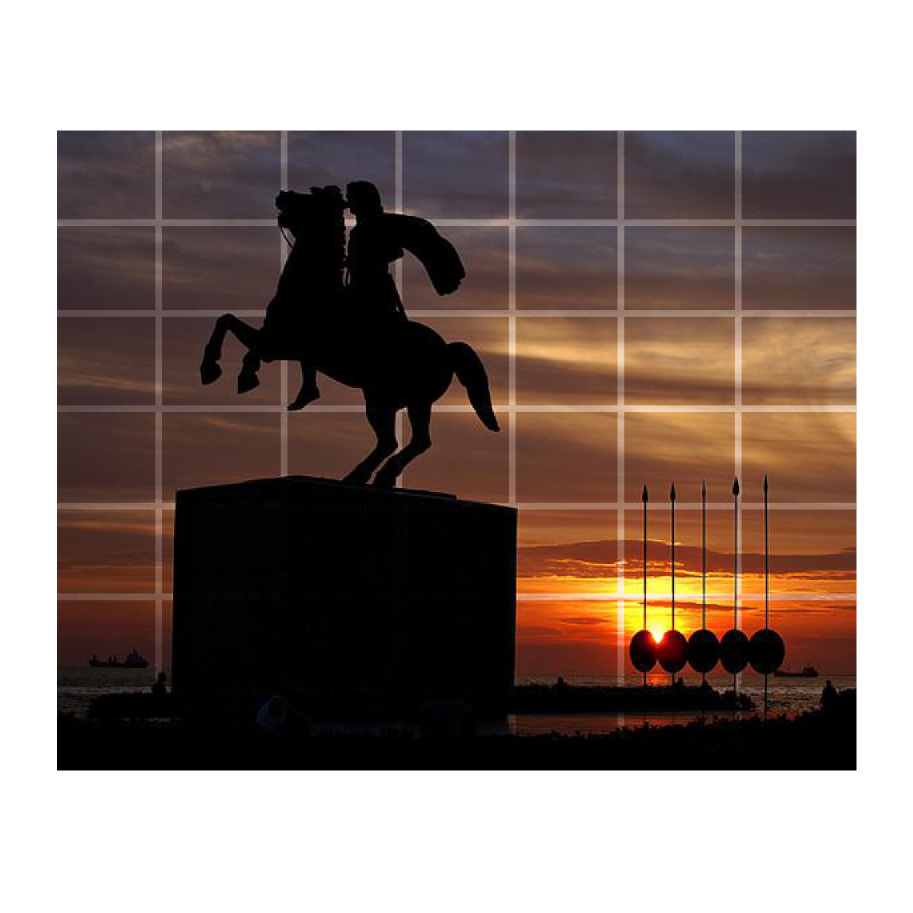
\includegraphics[width=0.5\textwidth]{process-image.png}
\caption{A Sunset Image Split into a 7x7 Grid}
\label{fig:process-image}
\end{figure}

\section{Experimental setup and results}
\label{sec:results}

\subsection{Input}
\begin{tabular}{ | c | c | c |}
\hline
 & Training & Test \\
\hline
Sunset & 223 & 254 \\
\hline
Non-Sunset & 276 & 245 \\
\hline
\end{tabular}

\subsection{SVM Parameter Results}
\subsubsection{Polynomial Kernel}
\begin{tabular}{ | c | c | c | c | c | c | c | c |}
\hline
p & TP & TN & FP & FN & TPR & FPR & Acc \\
\hline
2 & 211 & 226 & 19 & 43 & 83.07\% & 7.76\% & 87.58\% \\
\hline
3 & 218 & 239 & 6 & 36 & 85.83\% & 2.45\% & 91.58\% \\
\hline
4 & 211 & 222 & 23 & 43 & 83.07\% & 9.39\% & 86.77\% \\
\hline
5 & 206 & 240 & 5 & 48 & 81.10\% & 2.04\% & 89.38\% \\
\hline
6 & 196 & 131 & 114 & 58 & 77.17\% & 46.53\% & 65.53\% \\
\hline
\end{tabular}

\subsubsection{Radial Basis Function Kernel}
\begin{tabular}{ | c | c | c | c | c | c | c | c |}
\hline
\(\sigma\) & TP & TN & FP & FN & TPR & FPR & Acc \\
\hline
5 & 234 & 234 & 11 & 20 & 92.13\% & 4.49\% & 93.79\% \\
\hline
7 & 231 & 235 & 10 & 23 & 90.94\% & 4.08\% & 93.39\% \\
\hline
9 & 232 & 237 & 8 & 22 & 91.34\% & 3.27\% & 93.99\% \\
\hline
11 & 234 & 238 & 7 & 20 & 92.13\% & 2.86\% & 94.59\% \\
\hline
13 & 234 & 238 & 7 & 20 & 92.13\% & 2.86\% & 94.59\% \\
\hline
15 & 235 & 237 & 8 & 19 & 92.52\% & 3.27\% & 94.59\% \\
\hline
\end{tabular}

\section{Results of Various Sized Grid Runs}
\input{Results-Processed.txt}

\subsubsection{Summary}
The best accuracy came from the Radial Basis Function kernel with \(\sigma\) of 11, 13, and 15.  All three of these had identical accuracies.  The \(\sigma\)s of 11 and 13 were completely identical in their results, but the \(\sigma\) of 15 had one more true positive and one fewer true negative when compared to the other two.

None of the other grid sizes were able to give improved accuracy over the 7x7 grid, even losing accuracy in most cases.

\section{Conclusion}
We found that a basic technique using a 7x7 grid was able to classify the test set with greater than 94\% accuracy. Our normalization technique for normalizing the Y1 values greatly improved the accuracy of our code without requiring us to do manual threshold adjustments.

\subsection{Misclassifications}
Our classifier ended up misclassifying several images. The images that were false-positives typically contained hue and intensity values very similar to that of a sunset, such as evident by Figure \ref{fig:fp-1}, while false-negatives typically displayed low intensity values compared to other images in the data set.  

\begin{figure}
\centering
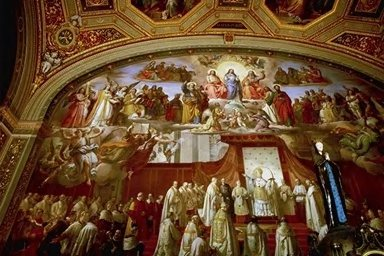
\includegraphics[width=0.5\textwidth]{fp-1.png}
\caption{A non-sunset misclassified as a sunset}
\label{fig:fp-1}
\end{figure}


\section{Future Work}
One possible area of future research would be to use other features aside from color to classify against, such as shape, edges, and color gradients.

One area that we would like to investigate in particular is dynamically determining the grid region sizes on an image-by-image basis. In addition, we would also like to investigate the use of irregularly sized grid regions. These regions would be optimized based on the training data and what would provide the smallest standard deviation of values within the region. 

Another area we would also like to investigate would be the possiblity of using multiple SVM models, each trained on a subset of sunset images, and combining the results to increase the accuracy and confidence of our system. 

\end{document}
